\cleardoublepage

\section{注意力机制图神经网络的多项式滤波设计方法}
本部分首先将介绍,图信号处理领域的近期研究结果,它将图卷积神经网络等效为低通滤波器[22]。受到它的启发,我们
接下来提出新的图卷积神经网络(poly GAT),并详细介绍我们设计的神经网络结构。

\subsection{低通滤波器}
近期的研究,有学者提出了一个基于图信号处理的分析图神经网络的理论框架。实验结果表明,图神经网络
只对输入信号进行低通滤波,不具有非线性流形学习的特征;他们还进一步研究了神经网络对噪声的适应能力,
并对基于GCN[23]的图神经网络设计提出了一些见解。
\subsubsection{图信号高频噪声假设}
    \textbf{假设1} \quad 输入的信号包含低频的真实信号和高频的噪声,真实信号能够为机器学习提供充分的信息。
    
    这个研究[22],在常用的数据集上验证了假设1。实验结果(图\ref{3-1})显示了将输入信号分解为不同频率的信号,然后分别用于
    两层感知器(MLP)的训练。在所有基准数据中,我们看到只有少量的频率成分有助于学习。当加入一
    些高斯噪声,在输入信号中加入更多的频率分量只会降低性能。
    \begin{figure}[ht]
        \centering
        \captionsetup{width=10cm}
        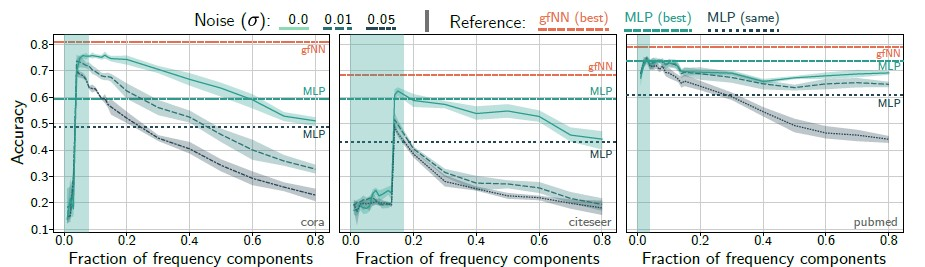
\includegraphics[width=17cm]{design/1.jpg}
        \caption{\label{3-1}对于Cora、citeseer、pubmed数据集,两层感知器(MLP)在不同频率的特征向量上的性能和gfNN网络最佳性能的对比}
    \end{figure}
    
    \textbf{假设2} \quad 
    观测到的特征信号${x(i)}_{i \in \nu}$包含了真实的信号${\bar{x}(i)}_{i \in \nu}$和噪声${z(i)}_{i \in \nu}$。
    真实信号$\bar{X}$的频率大多在$ 0 \le \epsilon \ll 1 $,噪声按照高斯白噪声分布,噪声$Z$的傅里叶变换的每一项都独立地
    服从正态分布$ N(0,\sigma^{2} ) $。

\subsubsection{理论推导}
可以认为$ X $已知,我们希望$ \hat{A}X $可以较精确地近似真值$ \bar{X} $,那么目标就是设计$ \hat{A} $。
接下来理论推导图卷积神经网络的效果,具体细节可见[22]。我们可以将两层感知器(MLP)表示为:
$$ h_{MLP}(X|W_1,W_2) = \sigma_{2}(\sigma_{1}(XW_1)W_2) $$
其中$\sigma_{1}$代表ReLU函数,$\sigma_{2}$代表softmax函数。$\sigma_{1}$和$\sigma_{2}$都是一种收敛的映射,
收敛映射的定义是$  \left \| \sigma_{i}(X)- \sigma_{i}(Y) \right \|_{D}  \le  \left \| X-Y \right \|_{D} $。

在假设1的前提下,我们的目标是获得与$ h_{MLP}(\bar{X}|W_1,W_2) $相类似的结果。最简单的方法是直接用观测到的特征信号,
来训练两层感知器$ h_{MLP}(X|W_1,W_2) $。这种方法的效果可以做以下估计:
$$  \left \| h_{MLP}(\bar{X}|W_1,W_2) - h_{MLP}(X|W_1,W_2) \right \|_{D}  \le  \left \| Z \right \|_{D} \rho(W_{1}) \rho(W_{2}) $$
其中$ \rho(W) $是$W$的最大特征值。

现在,我们不妨先使用图滤波器$ \hat{A}X $来估计特征信号,然后再用感知器$ h_{MLP}(\hat{A}X|W_1,W_2) $来训练,
通过推导我们可以得到以下结果:
$$  \left \| h_{MLP}(\bar{X}|W_1,W_2) - h_{MLP}(\hat{A}X|W_1,W_2) \right \|_{D}  =  \tilde{0}(\sqrt[]{\epsilon }) E[\left \| Z \right \|_{D}] \rho(W_{1}) \rho(W_{2}) $$

这意味着,如果真实数据的最大频率很小,我们可以用这种方法得到一个近似于最优的解决方案。

\subsubsection{阶段性结论与启发}
\begin{itemize}
    \item \textbf{结论} \quad
    证明了将图信号与传播矩阵相乘,对应于图信号通过低通滤波器。此外,还证明了观测信号与低通滤波器之间的
    矩阵乘积,实际上是求真实信号估计问题的解析解。从图信号处理理论的角度,我们的结果表明
    图卷积层的设计,某种程度上就是低通滤波器的设计。
    
    \item \textbf{启发} \quad
    基于这种理论理解,这个研究提出了一个新的图过滤神经网络框架gfNN来处理节点分类问题。
    gfNN网络包括两个步骤:1.与图滤波矩阵相乘来过滤得到真实信号;2.通过机器学习模型来学习节点标签。
    gfNN神经网络结构与传统GCN神经网络结构对比,如图\ref{3-2}所示。这样的设计思路,也可以应用到我们后续的设计当中。
    \begin{figure}[ht]
        \centering
        \captionsetup{width=10cm}
        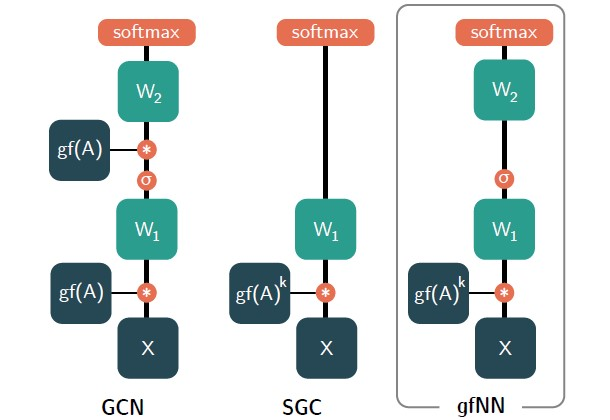
\includegraphics[width=10cm]{design/2.jpg}
        \caption{\label{3-2}GCN、SGC、gfNN 三种图卷积神经网络结构对比}
    \end{figure}
\end{itemize}

\subsection{poly GAT的结构}
由于效率、通用性和灵活性问题,空间模型在大多数场合比频谱模型更受欢迎。注意力机制图神经网络(GAT)
是一种最为通用的空间模型,其结构如图\ref{3-3}所示,我们将基于GAT来提出我们新的图卷积神经网络(poly GAT)。

我们在第二章理论基础部分,曾提及GAT神经网络的特点,现再对其主要缺点做简单总结。首先,是注意力
矩阵$A$必须1-hop的,如果直接将其变成2-hop将出现严重的过拟合现象,这使得其不能表示间接相连节点之间的关系;
其次,通常情况下GAT需要训练两个注意力矩阵$A_1$和$A_2$,这使得GAT需要较长的时间来训练网络,
然而如果只使用一个注意力矩阵,它的表达能力又将会大打折扣。

为了解决上述两个问题,我们融合了频谱理论,提出了新的图卷积神经网络(poly GAT),如图\ref{3-4}所示。
接下去,我们将详细介绍poly GAT的神经网络结构。

% \begin{figure}[htbp]
%     \centering
%     \begin{minipage}[t]{0.48\textwidth}
%     \centering
%     \captionsetup{width=5cm}
%     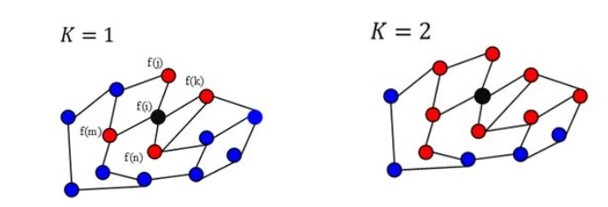
\includegraphics[width=8cm]{design/3.jpg}
%     \caption{\label{3-3}传统的GAT}
%     \end{minipage}
%     \begin{minipage}[t]{0.48\textwidth}
%     \centering
%     \captionsetup{width=5cm}
%     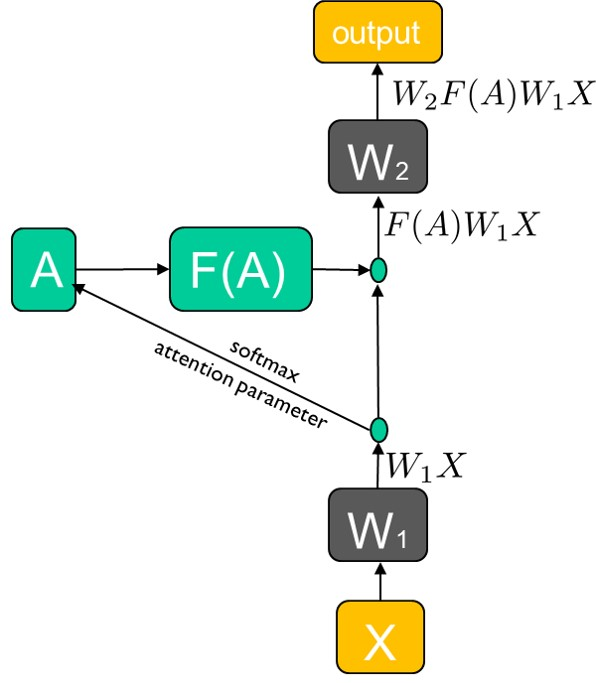
\includegraphics[width=8cm]{design/4.jpg}
%     \caption{\label{3-4}我们提出的poly GAT}
%     \end{minipage}
% \end{figure}

\begin{figure}[htbp]
    \centering
    \captionsetup{width=10cm}
    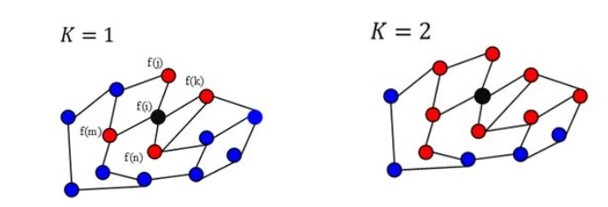
\includegraphics[width=11cm]{design/3.jpg}
    \caption{\label{3-3}传统的GAT}
\end{figure}

\begin{figure}[htbp]
    \centering
    \captionsetup{width=10cm}
    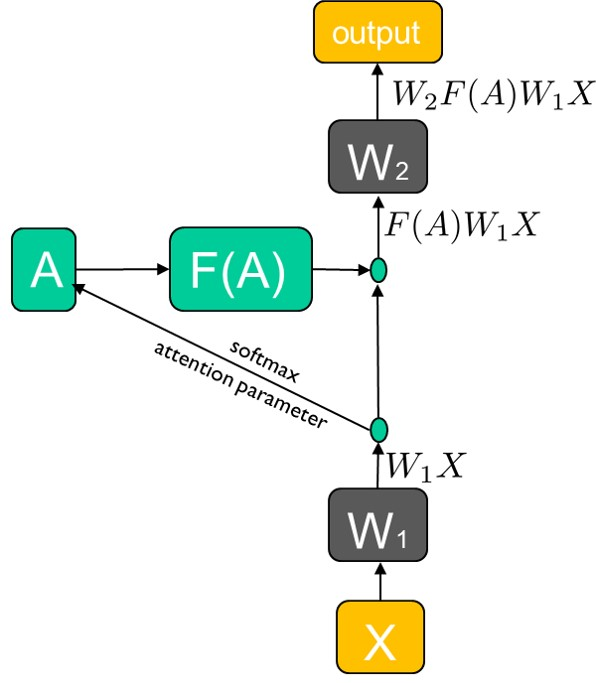
\includegraphics[width=13cm]{design/4.jpg}
    \caption{\label{3-4}我们提出的poly GAT}
\end{figure}

\subsubsection{步骤一:线性变换}
步骤一,如图\ref{3-5}所示,输入的特征信号$ X \in R^{F \times N} $,通过待训练的权重矩阵$ W_1 \in R^{F' \times F} $,输出的
信号为$ W_{1}X \in R^{F' \times N} $。其作用主要是通过线性变换对输入信号降维和特征提取。因为节点上的输入信号有时会
有很高的维度,如在cora数据集中$ F = 1433 $,过高的特征维度会给后续的滤波和机器学习带来困难,所以这一步
我们使用权重矩阵$ W_1,\in R^{F' \times F}, F' \ll F $来对输入信号的维度进行压缩和特征提取。
\begin{figure}[ht]
    \centering
    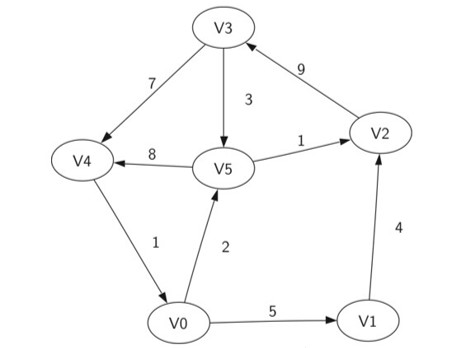
\includegraphics[width=2cm]{design/5.jpg}
    \caption{\label{3-5}步骤一}
\end{figure}

\subsubsection{步骤二:注意力机制}
步骤二,如图\ref{3-6}所示,输入的信号为$ W_{1}X \in R^{F' \times N} $,利用注意力参数$ \vec{a} \in R^{2F'} $,得到注意力矩阵
$A \in R^{N \times N}$。这一步的实现和GAT类似,主要作用是训练得到边权重(或称之为注意力权重)。注意力权重$A_{ij}$衡量节点$i$和
它相邻节点$j$的连接权重,对于不相邻的节点,$A_{ij} = 0$,对于相邻的节点,$ A_{ij} = \frac{exp(L(\vec{a}^{T}[W_{1}\vec{x_{i}}||W_{1}\vec{x_{j}}]))} { {\textstyle \sum_{k\in N_{i} }^{}} exp(L(\vec{a}^{T}[W_{1}\vec{x_{i}}||W_{1}\vec{x_{k}}]))} $
,$L$表示LeakyReLU。相较于直接学习每条边的权重,借助注意力参数$ \vec{a} \in R^{2F'} $间接的生成边权重,减少了参数量,有效地避免了过拟合。
\begin{figure}[ht]
    \centering
    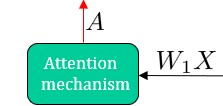
\includegraphics[width=4cm]{design/6.jpg}
    \caption{\label{3-6}步骤二}
\end{figure}

\subsubsection{步骤三:多项式滤波}
步骤三,如图\ref{3-7}所示,输入为注意力矩阵$A \in R^{N \times N}$,通过矩阵多项式$ F(A)={\sum_{i=1}^{K}c_{i}A^{i}} $ ,得到新的矩阵
$F(A) \in R^{N \times N}$。这一步,是我们设计的图卷积神经网络的主要创新,将频谱理论中使用矩阵多项式的设计方法应用到GAT中来。
我们在第二章理论基础中提到,GAT的图结构必须是1-hop,矩阵多项式使得我们自由选择图的hop。这是因为虽然注意力矩阵$A$的hop=1,
但是它是自连的,所以它的矩阵多项式$ F(A) $的hop值为$K$,这表明了不仅仅图上的相邻节点有连接权重,
间接相连的节点同样有连接权重,这将大大增强图卷积神经网络的表达能力。
\begin{figure}[ht]
    \centering
    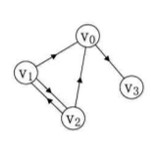
\includegraphics[width=4cm]{design/7.jpg}
    \caption{\label{3-7}步骤三}
\end{figure}

\subsubsection{步骤四:全连接层}
步骤四,如图\ref{3-8}所示,输入为经过滤波器$ F(A) $后的信号$ F(A)W_{1}X $,通过待训练的全连接层$ W_2 \in R^{F'' \times F'} $,
得到输出信号为$ W_{2}F(A)W_{1}X \in R^{F'' \times n} $。其作用是得到我们期望的节点分类的结果。与卷积神经网络(CNN)类似,
全连接层在整个网络中起到“分类器”的功能,将学到“分布式特征表示”映射到样本标记空间。即在图信号特征提取(滤波)之后,
我们需要通过全连接层得到我们期待的节点分类的结果。
\begin{figure}[ht]
    \centering
    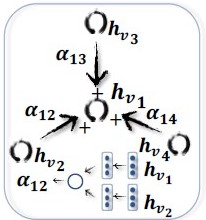
\includegraphics[width=4cm]{design/8.jpg}
    \caption{\label{3-8}步骤四}
\end{figure}

\subsection{设计思路总结}
总的来说,我们希望结合频谱模型和空间模型的设计方法,得到兼有其优点的图卷积神经网络。

\begin{itemize}
    \item \textbf{注意力机制} \quad
    将注意力机制应用于图卷积神经网络。不仅仅在图神经网络,注意力机制几乎在所有类型的神经网络都取得巨大的成功,简单
    的学习机制、较少的参数量、强大的表达能力,使得注意力机制成为了我们在设计复杂网络过程时的必然选择。此外,将注意力
    机制应用在图卷积神经网络的效果,在GAT中已经有了清楚体现,所以我们选择注意力机制来设计我们的滤波器。
    
    \item \textbf{矩阵多项式} \quad
    将矩阵多项式应用于图卷积神经网络。在频谱理论中,因为矩阵都是稀疏的,所以矩阵多项式能够使得图滤波器在很高的训练
    效率下,获得出色的拟合能力。此外,通过矩阵多项式还可以自由地选择图结构的hop,所以如果能将矩阵多项式应用图滤波器的
    设计,将在较小的训练代价下,使得神经网络的表达能力获得提高。

    \item \textbf{避免结构冗余} \quad
    相对于GAT网络,减少图滤波器的数量。在本章第一节,我们得到了相关的结论,图卷积神经网络的效果类似于图低通滤波器,且过多的低通滤波
    器不仅对滤波效果增强不大,还容易造成过拟合现象,所以gfNN网络仅用了一个低通滤波器就达到了理想的效果。如图3.3所示,
    GAT使用了$A_{1}$和$A_{2}$两个图滤波器,这对训练效率有很大的影响。所以如果图滤波器的数量存在冗余,我们需要合理地减少
    注意力矩阵的数量,进而提高训练效率。

\end{itemize}


